%%%%%%%%%%%%%%%%%%%%%%%%%%%%%%%%%%%%%%%%%%%%%%%%%%%%%%%%%%%%%%%%%%%%%%%%
% Escuela Politécnica Superior de la Universidad de Alicante
% Realizado por: Jose Manuel Requena Plens
% Contacto: info@jmrplens.com / Telegram:@jmrplens
%%%%%%%%%%%%%%%%%%%%%%%%%%%%%%%%%%%%%%%%%%%%%%%%%%%%%%%%%%%%%%%%%%%%%%%%


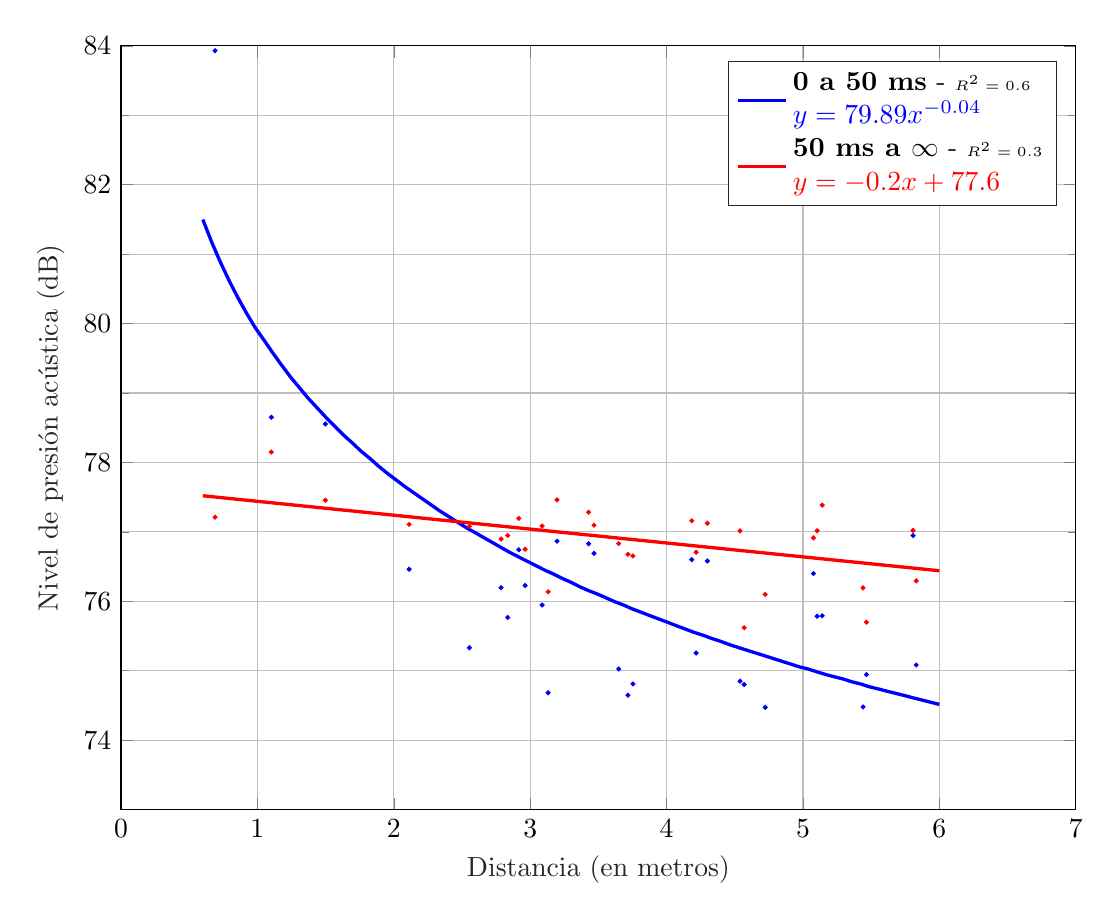
\begin{tikzpicture}

\begin{axis}[%
width=\textwidth,
height=0.8\textwidth,
at={(0\textwidth,0\textwidth)},
scale only axis,
xmin=0,
xmax=7,
xlabel style={font=\color{white!15!black}},
xlabel={Distancia (en metros)},
ymin=73,
ymax=84,
xmajorgrids,
xminorgrids,
ymajorgrids,
yminorgrids,
minor y tick num= 1,
ylabel style={font=\color{white!15!black}},
ylabel={Nivel de presión acústica (dB)},
axis background/.style={fill=white},
legend style={legend cell align=left, align=left, draw=white!15!black}
]
\addplot [color=blue, only marks,mark size=0.7pt, forget plot]
  table[row sep=crcr]{%
0.689492567037533	83.9298147556326\\
1.10208892563169	78.6508839586394\\
1.49833240637717	78.5537850719206\\
2.11248668634857	76.4616696030503\\
2.5540947515705	75.3307670198302\\
2.78664673039121	76.1965578400623\\
2.83511904511963	75.7676896799252\\
2.91626473421053	76.7421442885895\\
2.9626170862938	76.2279520874836\\
3.08787953132891	75.946910653961\\
3.13169283295792	74.682472152864\\
3.19677962956473	76.8654178100693\\
3.428206528201	76.8298033992244\\
3.46772259559498	76.6907385817452\\
3.64836949883095	75.0265374586113\\
3.71663826596024	74.6483005887243\\
3.75311870315875	74.8106601341298\\
4.18442349673165	76.6001904524153\\
4.21685902064559	75.2548274781649\\
4.29941856534113	76.5801826216203\\
4.53878838458019	74.8502307135703\\
4.56870878914383	74.8015849348429\\
4.72298634340605	74.4730406896843\\
5.07690850813761	76.4002346735743\\
5.10367514640186	75.7856409590404\\
5.14125471067132	75.7915936696579\\
5.44027572830643	74.4783975819506\\
5.46526303118158	74.9451316191164\\
5.80710771382795	76.9464967378256\\
5.83052313261855	75.0825990403115\\
};

\addplot[color=blue,domain=0.6:6, samples=85,line width=1.2]{79.89*x^(-0.039)};
\addlegendentry{\textbf{0 a 50 ms} - \tiny{$R^2 = 0.6$}\\$\color{blue}y = 79.89·x^{-0.04}$}


\addplot [color=red, only marks,mark size=0.7pt, forget plot]
  table[row sep=crcr]{%
0.689492567037533	77.2116251901105\\
1.10208892563169	78.1487656108054\\
1.49833240637717	77.4554982654753\\
2.11248668634857	77.1079070401778\\
2.5540947515705	77.0793479410879\\
2.78664673039121	76.8967227680043\\
2.83511904511963	76.9480634611297\\
2.91626473421053	77.1929999186771\\
2.9626170862938	76.7497664684574\\
3.08787953132891	77.0846862461668\\
3.13169283295792	76.136335003754\\
3.19677962956473	77.4614429688778\\
3.428206528201	77.2839536491472\\
3.46772259559498	77.0950077390861\\
3.64836949883095	76.8304860918788\\
3.71663826596024	76.6765715504004\\
3.75311870315875	76.6532524648088\\
4.18442349673165	77.1602815406925\\
4.21685902064559	76.7070937423991\\
4.29941856534113	77.1239304562105\\
4.53878838458019	77.0144084058593\\
4.56870878914383	75.6204899031107\\
4.72298634340605	76.0991888395833\\
5.07690850813761	76.9133557074926\\
5.10367514640186	77.0156266301233\\
5.14125471067132	77.3844643413919\\
5.44027572830643	76.1925753967431\\
5.46526303118158	75.6991412964459\\
5.80710771382795	77.0214783572162\\
5.83052313261855	76.2932567913482\\
};
\addplot[color=red,domain=0.6:6, samples=85,line width=1.2]{-0.2*x+77.64};
\addlegendentry{\textbf{50 ms a $\infty$} - \tiny{$R^2 = 0.3$}\\$\color{red}y = -0.2·x+77.6$}

\end{axis}
\end{tikzpicture}%